\chapter{Netzwerke}
\renewcommand{\chaptertitle}{Netzwerke}

\lehead[]{\sf\hspace*{-2.00cm}\textcolor{white}{\colorbox{lightblue}{\makebox[1.60cm][r]{\thechapter}}}\hspace{0.17cm}\textcolor{lightblue}{\chaptertitle}}
\rohead[]{\textcolor{lightblue}{\chaptertitle}\sf\hspace*{0.17cm}\textcolor{white}{\colorbox{lightblue}{\makebox[1.60cm][l]{\thechapter}}}\hspace{-2.00cm}}
%\chead[]{}
\rehead[]{\textcolor{lightblue}{AvHG, Inf, My}}
\lohead[]{\textcolor{lightblue}{AvHG, Inf, My}}


\section{Netzwerk-Kommunikation}

Heute ist es eine Selbstverständlichkeit, dass Computer miteinander vernetzt
sind. Das macht natürlich nur Sinn, wenn Programme diese Netzwerkverbindungen
nutzen. Etwa für e-Mail-Kommunikation, Online-Banking oder Zugriff auf das WWW.

Bei der Netzwerk-Kommunikation von Programmen wird zwischen zwei Modellen
unterschieden: Dem sogenannten \emph{Client-Server-Modell} und dem
\emph{Peer-to-Peer-Modell}.

\subsection{Peer to Peer (P2P)}

Im Peer-to-Peer-Modell sind alle Kommunikationspartner (Programme)
gleichberechtigt. Es gibt keine Aufgabentrennung und jeder Teilnehmer kann
-- zumindest potentiell -- direkt mit jedem anderen Teilnehmer kommunizieren.

Man spricht deshalb auch vom \emph{symmetrischer Kommunikation}.

\begin{minipage}{0.5\textwidth}
\begin{center}
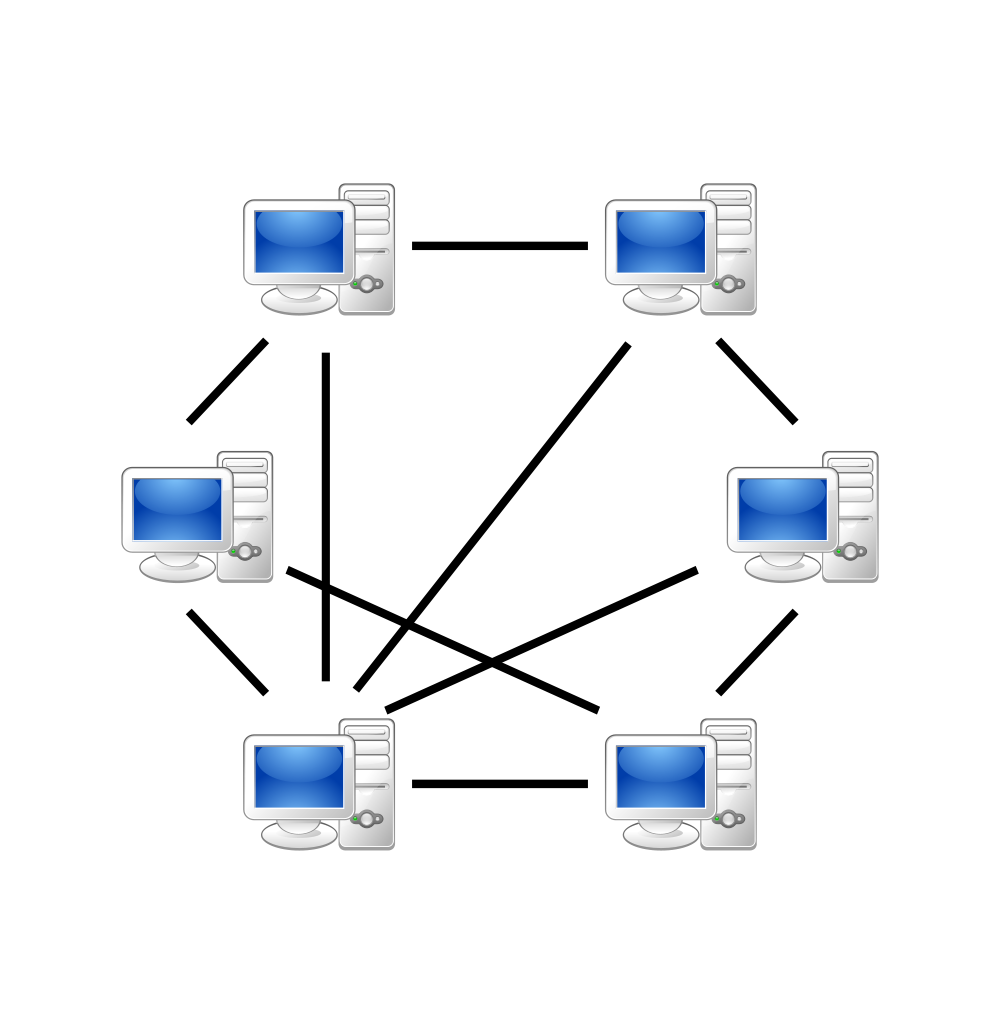
\includegraphics[width=0.8\textwidth]{./inf/SEKII/42_Netzwerke/P2P.png}
% http://commons.wikimedia.org/wiki/File:P2P-network.svg
% Public Domain

Peer-to-Peer-Modell
\end{center}
\end{minipage}
\begin{minipage}{0.5\textwidth}
\begin{center}
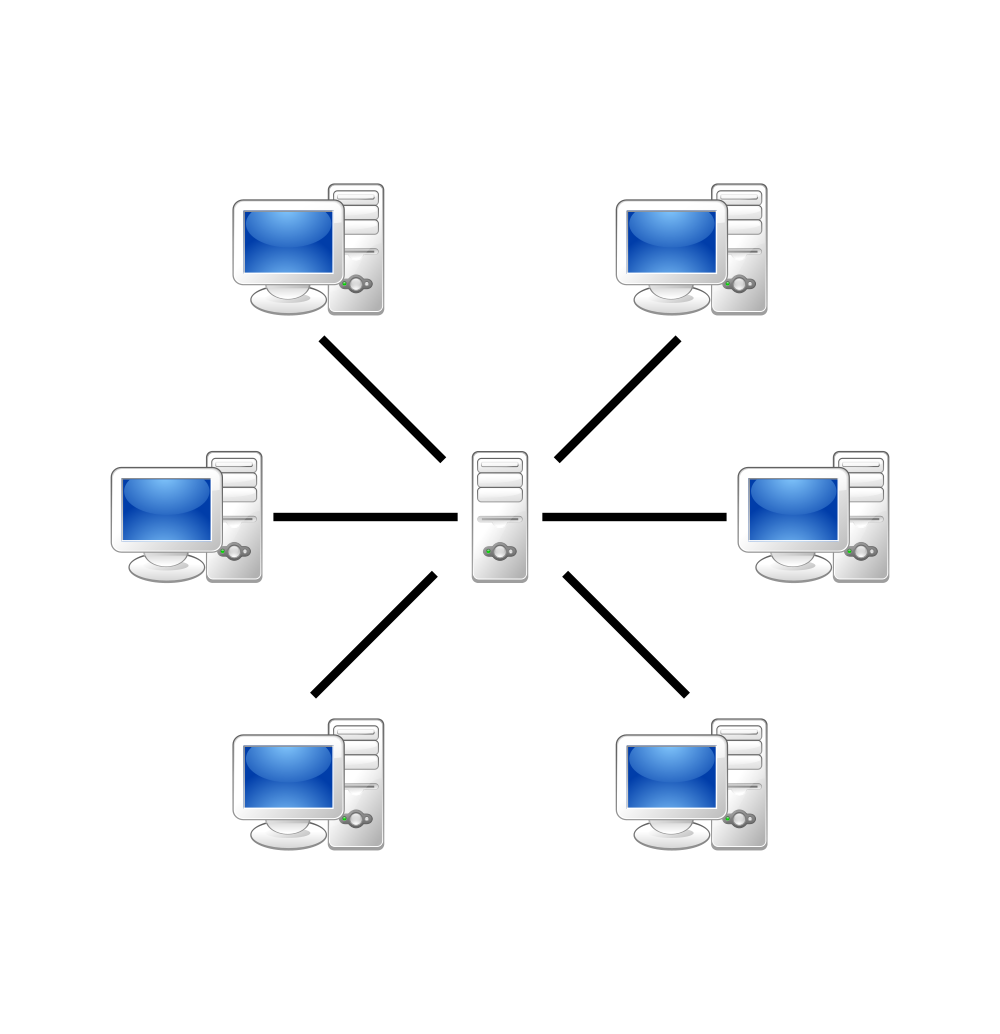
\includegraphics[width=0.8\textwidth]{./inf/SEKII/42_Netzwerke/CS.png}
% http://commons.wikimedia.org/wiki/File:Server-based-network.svg
% LGPL

Client-Server-Modell
\end{center}
\end{minipage}


\subsection{Client-Server}

Der Gegensatz zum Peer-to-Peer-Modell ist das Client-Server-Modell. Bei diesem
bietet ein \emph{Server} einen Dienst an und ein \emph{Client} nutzt diesen
Dienst.

Ein Web-Server zum Beispiel ist ein Programm, das HTML-Seiten zur Verfügung
stellt. Der Web-Server nimmt Anfragen von Browsern (den Web-Clients) entgegen
und schickt ihnen anschließend das gewünschte Dokument.

Die Bezeichnungen Client und Server werden häufig auch für Computer verwendet.
Ein Computer wird als Server bezeichnet, wenn auf ihm ein Server-Programm
läuft. Ein Computer wird als Client bezeichnet, wenn auf ihm Client-Software
ausgeführt wird. Da auf einem Computer gleichzeitig sowohl Server- als auch
Client-Programme laufen können ist diese begriffliche Zuordnung nicht immer
eindeutig. So läuft beispielsweise auf jedem Rechnern in unserem Informatik-Raum
ein Datenbank-Server aber auch verschiedene Clients.


\section{Protokoll}

Wenn Computer über das Netzwerk Daten austauschen sollen, muss vorher genau
definiert werden, welche Daten in welcher Reihenfolgen zu senden sind, damit
die Computer sich auch richtig verstehen. Die festgelegten Regeln, die
notwendig sind, um einen kontrollierten und eindeutigen Verbindungsaufbau,
Datenaustausch und Verbindungsabbau zwischen zwei Rechnern zu gewährleisten
bezeichnet man als \emph{Protokoll}. Das Protokoll ist für Computer genauso wie
für Diplomaten die Summe der Umgangsformen. Wer sich an die vereinbarten Regeln
hält, wird verstanden.


\section{OSI-Schichtenmodell}

Wenn ein einziges Programm alle Aufgaben übernehmen sollte, die zur Übertragung
von Daten über das Netz notwendig sind, wäre dieses Programm so komplex, dass
die zuständigen Programmierer im wahrsten Sinne des Wortes verrückt werden
würden. Um die Komplexität zu bewältigen hat man deshalb die Aufgaben in
verschiedene Teilbereiche unterteilt, die einzeln programmiert werden und
aufeinander aufsetzen -- eine Art \glqq Baukastensystem\grqq . 1983 wurde von
der Internationalen Standard Organisation (ISO) das berühmte
\emph{OSI-Schichtenmodell} festgelegt, dass sieben verschiedene \glqq
Bauteile\grqq\ (Schichten) definiert:

\begin{center}
\begin{minipage}{0.9\textwidth}
\bgroup
\def\arraystretch{1.2}
\begin{tabularx}{\textwidth}{|p{20mm}|X|}
\hline
\textbf{Schicht 7} &
\textbf{\emph{Anwendungsschicht -- Application Layer}}

Anwendungsprogramme: e-Mail, Browser, Dateitransfer
\\ \hline
\textbf{Schicht 6} &
\textbf{\emph{Darstellungsschicht -- Presentation-Layer}}

Konvertierung von Darstellungsformaten, zum Beispiel ASCII, EBCDIC, UTF
\\ \hline
\textbf{Schicht 5} &
\textbf{\emph{Sitzungsschicht -- Session Layer}}

Kommunikation von Sitzungen in Multi-User-Umgebungen
\\ \hline
\textbf{Schicht 4} &
\textbf{\emph{Transportschicht -- Transport Layer}}

Aufteilung bzw. Zusammensetzung von Daten in Pakete
\\ \hline
\textbf{Schicht 3} &
\textbf{\emph{Vermittlungsschicht -- Network Layer}}

Auswahl der Übertragungswege für Datenpakete
\\ \hline
\textbf{Schicht 2} &
\textbf{\emph{Sicherungsschicht -- Data Link Layer}}

Ver- und Entpacken der Datenpakete für das genutzte Medium
\\ \hline
\textbf{Schicht 1} &
\textbf{\emph{Bitübertragungsschicht -- Physical Layer}}

Festlegung der elektrischen und mechanischen Parameter einer Datenkommunikation
\\ \hline
\end{tabularx}
\egroup
\end{minipage}
\end{center}

Siehe \url{http://de.wikipedia.org/wiki/OSI-Modell}


\section{TCP/IP im vereinfachten Schichtenmodell}

Für die Internet-Protokolle (TCP/IP) wird häufig ein vereinfachtes
Schichtenmodell mit vier Ebenen benutzt:

\begin{center}
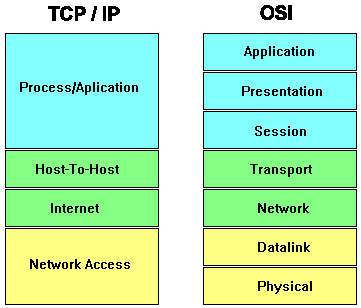
\includegraphics[width=0.5\textwidth]{./inf/SEKII/42_Netzwerke/tcpipiso.png}
% http://www.netzmafia.de/skripten/netze/netz0.html
% Anfrage per e-Mail am 25.3.

Grafik entnommen von \url{http://www.netzmafia.de/skripten/netze/netz8.html}
\end{center}

Für die \emph{physikalische Schicht} kommen je nach verwendeter Hardware sehr
unterschiedliche Protokolle zum Einsatz (zum Beispiel Ethernet, ATM, usw.). Die
Protokolle auf dieser Ebene wissen wie die spezielle Hardware angesprochen
werden muss und können Datenpakete zwischen zwei Rechnern austauschen.

Auf der \emph{Netzwerkschicht} wird in Internet-basierten Netzen immer das
\emph{IP-Protokoll} verwendet. Das IP-Protokoll verwaltet unter anderem die
Adressen der Rechner und ermöglicht so die Übertragung eines Datenpakets durch
das Netz zu einem bestimmten Zielrechner.

Die \emph{Transportschicht} übernimmt die Adressierung des Prozesses auf einem
Rechner und vergibt dazu sogenannte \emph{Port-Nummern}. Damit gelangen
übertragene Datenpakete nicht nur an den richtigen Rechner, sondern auch zu der
Anwendung, für die sie gedacht sind. Dafür stehen zwei verschiedene Protokolle
zur Verfügung:

\begin{compactitem}
\item Das \emph{TCP-Protokoll} teilt die Daten eines Anwendungsprogramms in
Datenpakete auf und übergibt sie zur Übertragung an das IP-Protokoll. Auf der
Empfänger-Seite sorgt TCP dafür, dass die Daten aus den einzelnen Paketen in
der richtigen Reihenfolge wieder zusammen gesetzt werden und verloren gegangene
Pakete erneut gesendet werden. 
\item Alternativ kann man das \emph{UDP-Protokoll} verwenden, das jedoch weit
weniger Funktionalität besitzt als TCP. Bei Verwendung des UDP-Protokolls muss
das Anwendungsprogramm seine Daten selber in Datenpakete aufteilen. Das
UDP-Protokoll stellt auch nicht sicher, dass die Datenpakete bei Fehlern erneut
gesendet werden. Um verloren gegangene Datenpakete muss sich die Anwendung
selber kümmern.
\end{compactitem}

Auf oberster Ebene stehen die Protokolle für die verschiedenen Anwendungen
(zum Beispiel FTP zum Filetransfer, SMTP zum Mail-Versand oder HTTP zur
Übertragung von Web-Seiten). Für Spezial-Anwendungen kann jeder Programmierer
ein eigenes Protokoll entwickeln.

Wenn das Anwendungsprogramm Daten übertragen möchte, werden nacheinander die
einzelnen Protokoll-Schichten aufgerufen und jede Schicht packt zu dem
Datenpaket eigene Daten hinzu, die sie für ihre Verwaltungsarbeit benötigt:

\begin{center}
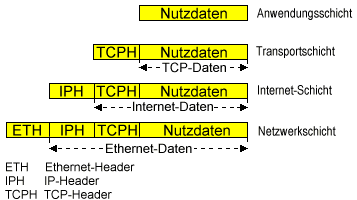
\includegraphics[width=0.6\textwidth]{./inf/SEKII/42_Netzwerke/schichten.png}
% http://www.netzmafia.de/skripten/netze/netz0.html
% Anfrage per e-Mail am 25.3.

Grafik entnommen von \url{http://www.netzmafia.de/skripten/netze/netz8.html}
\end{center}

Das einfache UDP-Protokoll erzeugt zum Beispiel für jedes Datenpaket einen
zusätzlichen \emph{Header} mit folgendem Format:

\begin{center}
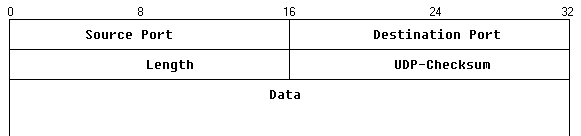
\includegraphics[width=0.75\textwidth]{./inf/SEKII/42_Netzwerke/udp.png}
% http://www.netzmafia.de/skripten/netze/netz0.html
% Anfrage per e-Mail am 25.3.

Grafik entnommen von \url{http://www.netzmafia.de/skripten/netze/netz8.html}
\end{center}

\begin{compactitem}
\item[\textbf{Source Port:}] Identifiziert den sendenden Prozess. 

\item[\textbf{Destination Port:}] Identifiziert den Prozess des Zielknotens. 

\item[\textbf{Length:}] Länge des UDP-Datagramms in Bytes (mindestens 8 =
Headerlänge)

\item[\textbf{UDP-Checksum:}] Optionale Angabe einer Prüfsumme (falls nicht
verwendet auf Null gesetzt).
\end{compactitem}

Die Verwaltungsinformationen, die das TCP-Protokoll und das IP-Protokoll in
ihren Headern generieren, sind noch weit komplizierter.


\section{IP-Adressen}

Die vom IP-Protokoll vergebene IP-Nummer (od. IP-Adresse) ist die Adresse eines
Computers im Internet. Die IP-Adresse besteht aus einer weltweit einmaligen
32-Bit-Zahl. Die ersten Bits kennzeichnen die Klasse des Netzes, in dem sich
der Computer befindet: A (großes Netz), B (mittelgroßes Netz) oder C (kleines
Netz). Anschließend folgen Bits zur Identifikation des Netzes. Die restlichen
Bits identifizieren den jeweiligen Computer.

Zur leichteren Lesbarkeit werden die 32-Bit-Adressen in vier Bytes zerlegt und
durch Punkte getrennt dezimal dargestellt.

Bsp.: \lstinline|193.246.253.248|

Anmerkung: Hier wurde die heute noch gebräuchliche Version 4 (IPv4)
beschrieben. Der Adressraum ist bei IPv4 jedoch inzwischen deutlich zu klein,
so dass in den nächsten Jahren von IPv4 auf IPv6 umgestellt werden muss (die
Umstellung läuft bereits -- aber so lange noch nicht alle Teilnehmer im Internet
mit IPv6 umgehen können wird parallel weiterhin auch mit IPv4 gearbeitet). Der
Adressraum von IPv6 ist so riesig ($3.4 \cdot 10^38$ Adressen statt $4.3 \cdot
10^9$ Adressen bei IPv4), dass man theoretisch jedem Molekül im Universum seine
eigene IP-Adresse geben könnte. IPv6 Adressen sehen etwas anders aus:

\begin{lstlisting}
> host heise.de
heise.de has address 193.99.144.80
heise.de has IPv6 address 2a02:2e0:3fe:100::8
\end{lstlisting}
 
\section{Host- und Domain-Namen}

Wir Menschen können uns IP-Nummern äußerst schlecht merken. Darum dürfen
Computer auch Namen besitzen. 

Als \emph{Host} wird der Name des Rechners bezeichnet, Als \emph{Domainname} der
Rest der Adresse. Ein Beispiel: \myUserInput{pop3.web.de} –- \myUserInput{pop3}
ist der Hostname und \myUserInput{web.de} der Domainname.
Das Ganze (\myUserInput{pop3.web.de}) wird auch als \emph{Fully Qualified Domain
Name} (FQDN) bezeichnet.

Um zwischen dem für uns Menschen und den für die Adressierung tatsächlich verwendeten
numerischen IPs hin und her übersetzen zu können braucht es einen Dienst: den
\emph{Domain Name Service} (DNS). Ein Rechner, der diesen Dienst anbietet wird
\emph{DNS-Server} genannt.

Die Zuordnung IP $\leftrightarrow$ FQDN ist nicht eindeutig. In keine Richtung!
Zu einer IP gehören oft mehrere FQDNs, da auf einem Server oft mehrere Dienste
angeboten werden (z.B.\ \myUserInput{www.example.com} für den HTTP-Server,
\myUserInput{smtp.example.com} für den SMTP-Server). Außerdem werden von großen
Hostern aber auch innerhalb von Firmen oft mehrere Webserver virtuell auf dem
gleichen physikalischen Server angeboten. 

\begin{lstlisting}
> host www.humboldtgymnasium-bremen.de
www.humboldtgymnasium-bremen.de has address 89.31.143.7
> host www.gabys-modewelt.de
www.gabys-modewelt.de has address 89.31.143.7
> host www.waldorfschule-hassfurt.de
www.waldorfschule-hassfurt.de has address 89.31.143.7
> host www.sommerbadminden.de
www.sommerbadminden.de has address 89.31.143.7
\end{lstlisting}

(Es gibt noch viele weitere Webseiten, die alle auf dem selben Webserver
gehostet sind wie unsere Schul-Homepage und deshalb auch alle auf die gleiche
IP-Nummer zeigen)

In diesem Fall lässt sich der Webserver übrigens auch nicht über die IP
adressieren: Zwar kommt die Verbindung zustande, aber der Server weiß ja nicht
für welche der Domains, für die er zuständig ist, er Daten ausliefern soll.

Umgekehrt „verstecken“ sich hinter einem FQDN oft auch mehrere physikalische
Server. Das kann zum einen zur Steigerung der Ausfallsicherheit wünschenswert
sein, aber oft auch allein schon um den möglichen Durchsatz zu steigern. Oder
könnt ihr euch vorstellen, dass hinter \myUserInput{www.google.com} nur ein
einziger physikalischer Server hängt?

\begin{lstlisting}
> host www.google.com
www.google.com has address 173.194.112.16
www.google.com has address 173.194.112.17
www.google.com has address 173.194.112.18
www.google.com has address 173.194.112.19
www.google.com has address 173.194.112.20
www.google.com has IPv6 address 2a00:1450:4001:800::1014
\end{lstlisting}

Das geht sogar noch weiter: Stichwort \emph{Round Robin DNS}


\subsection{Loopback-Adresse}

Von besonderer Bedeutung für die Programmentwicklung ist die
\emph{Loopback-Adresse} \lstinline|127.0.0.1|, die mit dem Namen
\lstinline|localhost| bezeichnet wird.

Datenpakete mit dieser Klasse-A-Adresse treffen, ohne jemals auf das Netzwerk
zu gelangen, unmittelbar wieder beim sendenden Computer ein und können deshalb
zum Funktionstest bei der Programmierung von Internet-Anwendungen verwendet
werden. Oder um Programme auf dem lokalen Rechner über das TCP/IP-Protokoll zu
erreichen (etwa den bei uns lokal laufenden Datenbankserver).


\section{IP-Adressen in Java}

Zur Arbeit mit IP-Adressen wird die Klasse \myClass{InetAddress} des Pakets
\myPackage{java.net} verwendet. Um ein Objekt der Klasse \myClass{InetAddress}
zu generieren, ruft man die statische Methode
\lstinline|InetAddress.getByName()| auf und gibt als Parameter entweder eine
IP-Adresse oder den Domain-Namen an (beides als String):

\begin{lstlisting}
public static InetAddress getByName(String host) throws UnknownHostException
\end{lstlisting}

Wenn die Adresse vom DNS-Server nicht aufgelöst werden kann, wird eine
\myClass{UnknownHostException} geworfen. Diese Exception sollte man abfangen und
eine sinnvolle Fehlermeldung erzeugen.

Nachdem ein \myClass{InetAdress}-Objekt generiert wurde, kann man mit den beiden
folgenden Methoden den Domain-Namen und die IP-Adresse des Rechners ermitteln:

\begin{lstlisting}
String getHostName()      æ// gibt den Domain-Namen zurück
æString getHostAddress()   æ// gibt die IP-Adresse zurück (als String)
\end{lstlisting}

Beispiel-Code (Auszug):

\begin{lstlisting}
import java.net.*;
æ...
æString eingabe = "127.0.0.1";
InetAddress inet = InetAddress.getByName(eingabe);
String host = inet.getHostName();        æ// Rückgabe: "localhost"
æString ip = inet.getHostAddress();	     æ// Rückgabe: "127.0.0.1"
\end{lstlisting}
		

\section{Port-Nummern}

Da häufig mehrere Server auf einem Rechner laufen, reicht für die Kommunikation
die IP-Adresse des Rechners nicht aus. Das TCP-Protokoll übernimmt die
Adressierung der Anwendungen auf einem Rechner und vergibt dazu sogenannte
Port-Nummern, die zwischen 0 und 65535 liegen. Portnummern im Bereich von 0 bis
1023 sind für Anwendungen mit Administratorrechten reserviert. Für bekannte
Internet-Dienste gibt es festgelegte Portnummern (\emph{Well Known Ports}).
Beispiel:

\begin{center}
\begin{minipage}{0.95\textwidth}
\bgroup
\def\arraystretch{1.2}
\begin{tabularx}{\textwidth}{|X|X|X|X|}
\hline
\textbf{Internet-Dienst} &
FTP (Filetransfer) & HTTP (Web-Server) & SMTP (Mail-Versand)
\\ \hline
\textbf{Portnummer} &
21 & 80 & 25
\\ \hline
\end{tabularx}
\egroup
\end{minipage}
\end{center}